\documentclass[/home/greg/Thesis/main/main.tex]{subfiles}

\begin{document}

\graphicspath{{/home/greg/Neutron_star_modelling/SpindownRate/img/}}
\inputpath{/home/greg/Neutron_star_modelling/SpindownRate/}

\newcommand{\spindown}{\dot{\nu}}
\newcommand{\Aem}{\mathcal{A}_{\mathrm{EM}}}
\section{Physical observables: spin-down rate $\spindown$}

An observable which is often considered in characterising periodic patterns in
pulsar signals is the spin-down rate $\spindown$. In our numerical model, the
spin-down rate is the same as the second derivative of the magnetic dipoles 
azimuthal angle (i.e. $\ddot{\Phi}$). 

As we will now show, the spin-down rate is modulated by free precession, but
this effect can also be amplified by the electromagnetic torque as first shown
by \citet{Jones2004}. In order to understand all of the subtle physics which
may be present in the spin-down rate, we will now build our intuition by starting
with the simplest models and gradudally introducing new features. 

Calculation of the spin-down rate can be done in two ways: either analytically
building on results from \citet{Jones2004}, or we can numerically solve the
system of equations and measure the spin-down rate (discussed shortly). Using the
latter method we include by default all of the interplay between precession and
the EM torque. We then compare this `exact' solution with analytic results
which allows us to understand which parts of the system are responsible for the
observed phenomena. 

In order to measure the spin-down rate from numerical solutions we could
numerically differentiate eqn.~\eqref{eqn: Phi} (the angular phase of the
magnetic dipole). However, since we are comparing our results with measured
values from pulsar astronomers, an alternative is use the method proposed by
\citet{Lyne2010}: a second order Taylor expansions is fitted to short sections
of data of length $T$ and the resulting coefficient $\spindown$ is recorded the
mid-point in time of the section of data. Repeating this process every $\sim
T/4$ in a `sliding-window', we build a picture of how the spindown varies with time.
We choose $T$ such that it is a fraction of the precession period over which we
expect quantities to be modulated. This is consistent with the observers method
where $T$ is chosen in order to resolve the observed modulations, but average
out the short-time scale changes.

We now proceed to compare this numerical spin-down rate calculation with analytic
predictions gradually introducing new features when required. Since the geometric
variations can be quite complex, we consider only $\theta < \chi$ and start 
with $\theta \approx 3^{\circ}$ and $\chi=60^{\circ}$. This produces simple
simple oscialltory behaviour. The solution become more complex if either
the inequality is not satisfied or $\chi \approx \pi/2$ so we initially
ignore this region and return to it later on.

\subsection{Spin-down variations due to free-precession}
Without an EM torque, the average spin-down rate should be zero. However, if
the body undergoes free precession, this will produce periodic variations. These
can be calculated exactly by differentiating eqn. \eqref{eqn: Phi_dot}, because
the torque is zero we have $\dot{\theta} = 0$ leaving
\begin{equation}
    \ddot{\Phi}(t)_{\mathrm{p}} = \ddot{\phi} + \frac{d}{dt}\left(
        \sin\chi\dot{\psi} \frac{\cos\theta\sin\chi - \sin \psi \sin \theta \cos\chi 
}{(\sin\theta \cos \chi - \cos \theta \sin \psi \sin \chi)^{2} + \cos^{2}\psi \sin^{2} \chi}
\right)
\label{eqn: Phi_ddot FP}
\end{equation}
The resulting expression is unweildy and so we do not report it here. For a 
freely precessing biaxial body we demonstrated in section \ref{sec: Biaxial body with no torque}
that the euler angles are linear functions of time. As such the first term 
in this expression vanishes and we are left with a complicated trigonometric
function of $\psi(t)$ which is given by eqn. \eqref{eqn: euler angles torque free evolution}.

It is also useful to calculate the magnitude of variations: this is done by
differentiating equation \eqref{eqn: Jones 49} twice which gives:
\begin{equation}
    |\Delta\spindown|_{\mathrm{p}} =\frac{\dot{\psi}^{2} \theta \cot\chi}{2\pi}. 
    \label{eqn: spin-down variations FP}
\end{equation}

In figure \ref{fig: nu_dot no torque} we plot three curves: the numerical
result obtained using Lyne method of calculating the spin-down, the analytic
prediction from eqn.~\eqref{eqn: Phi_ddot} and the magnitude obtained by
eqn.~\eqref{eqn: spin-down variations FP}
\begin{figure}[ht]
\centering
	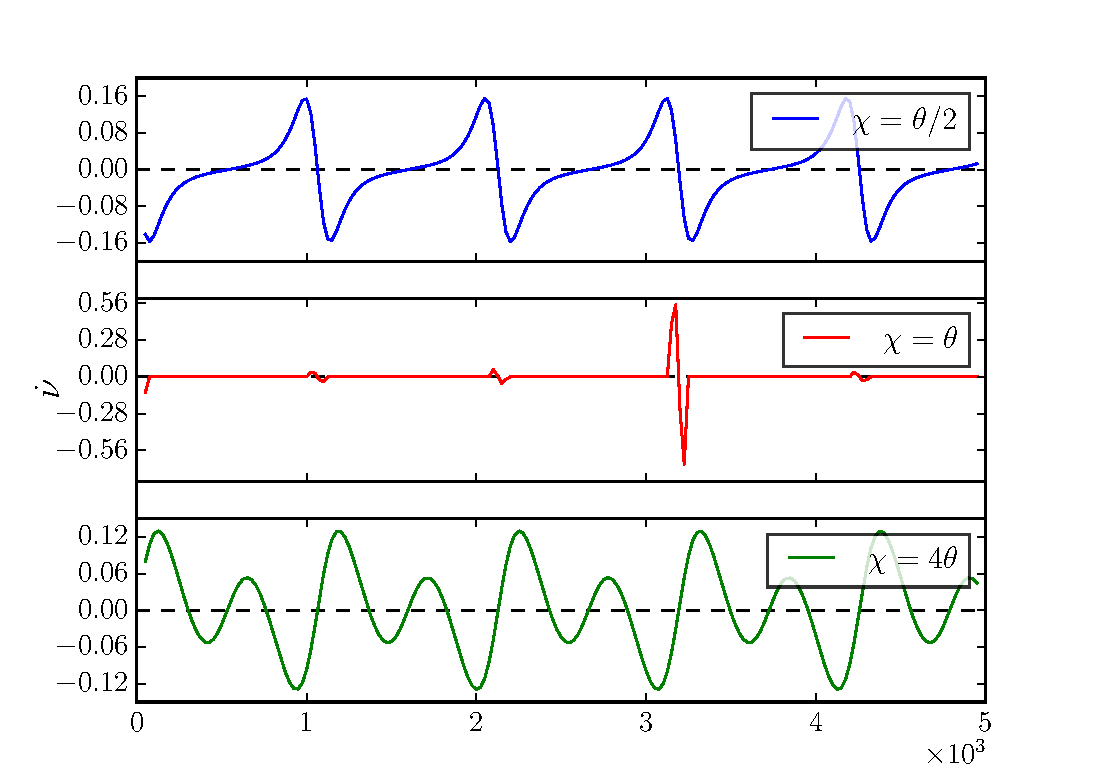
\includegraphics[width=0.5\textwidth]{nu_dot_no_torque.pdf}
\caption{Modulations in the spin-down rate due to free precesion. The solid black
         line is the numerical solution. in blue we show the analytic 
         preduction of the magnitude of modulations due to free-precession as
         given by equation \eqref{eqn: spin-down variations FP} and the red-dashed
         line indicates the analytic prediction of eqn~/\eqref{eqn: Phi_ddot}}
\label{fig: nu_dot no torque}
\end{figure}

The variations seen in figure \ref{fig: nu_dot no torque} are the result of
free precession. As there is no torque, the overall spindown is zero. However,
due to precession the magnetic dipole performs a slow rotation about the
deformation axis. During half the cycle it counter-rotates and in the other
half it corotates with the rapid rotation about the angular momentum vector.
The result is a symmetric modulation of the spindown about zero with magnitude
given by equation \eqref{eqn: spin-down variations FP}.

\subsection{Spin-down due to EM torque}
\subsubsection{Averaged spin-down rate}
When we include the EM torque we will have a non-zero average spin-down rate. 
We can measure this directly from equation \eqref{eqn: surface magnetic field}:
rearranging for $\dot{\Omega}$ we have
\begin{equation}
    \dot{\Omega} = -\frac{B_{0}^{2}R^{6} \sin^{2}\alpha \Omega^{3}}{6I_{0}c^{3}},
\end{equation}
writen in terms of the model parameters this is
\begin{equation}
\dot{\nu} = -\frac{1}{3\pi}\frac{R \Omega^{3}}{c} \sin^{2}\alpha \epsA
\end{equation}
In general the spin-down is approximately constant over a given observation
time. As a result we estimate the spin-down rate by the initial value:
\begin{equation}
    \dot{\nu}_{0} \approx -\frac{1}{3\pi}\frac{R \Omega_{0}^{3}}{c} \sin^{2}\alpha \epsA
    \label{eqn: spin-down initial EM}
\end{equation}
Here $\alpha$ is the angle between the spin-vector and the magnetic dipole. For
small wobble angles, the angle $\hat{\theta}$ (see figure \ref{fig: reference plane})
is vanishingly small and so we can approximate $\alpha \approx \chi$ such that
the spin-down is 
\begin{equation}
    \dot{\nu}_{0} = -\frac{1}{3\pi}\frac{R \Omega_{0}^{3}}{c} \sin^{2}\chi \epsA
    \label{eqn: spin-down initial EM chi}
\end{equation}

This expression will give us the average spin-down under an EM torque; if the
star precesses, then the actual spin-down will be modulated about this values
due to precession. Before demonstrating how to calculate this modulation we
first show that the magnitude of modulation will depend on the EM torque.

\subsubsection{Amplification of the spin-down modulation}
The magnitude of the spin-down modulation due to precession will 
depend on the EM amplification factor which we discussed in equation 
\eqref{eqn: EM amplification factor}. For the timing residuals \citet{Jones2001}
demonstrated that the residuals could be amplified by the EM torque, we now
show that a similar effect occurs for the 
spin-down modulation. Starting with a vacuum point-dipole spin-down torque
\begin{equation}
    \ddot{\Phi} = k\dot{\Phi}^{3}\sin^{2}\alpha,
\end{equation}
then \citet{Jones2001} demonstrated that the magnitude of modulations of the 
spin-down rate is
\begin{equation}
    |\Delta\ddot{\Phi}|^{58} \approx -2k\Omega^{3} \theta \sin\chi \cos\chi 
\end{equation}
here the superscript refers to the relevant equation in \citet{Jones2001}. Taking
this expression, we now show that it can be rewritten
\begin{align}
    |\Delta\ddot{\Phi}|^{58} 
    & \approx 2k\Omega^{3} \theta \sin\chi \cos\chi & \\
    & \approx 2 \frac{\ddot{\Phi}}{\sin^{2}\alpha} \theta \sin\chi\cos\chi &
    \mathrm{if }\; \alpha \approx \chi \\
    & \approx 2 \ddot{\Phi}\theta \cot\chi & 
    \tauS = \left| \dot{\Phi} / \ddot{\Phi}\right| \\
    & \approx 2 \frac{\dot{\Phi}}{\tauS} \theta \cot\chi &
    P/\tauP = \dot{\psi}/\dot{\Phi} \\
    & \approx 2 \dot{\psi}^{2}\left(\frac{\tauP}{P}\right) \frac{1}{\dot{\psi}} \frac{1}{\tauS} \theta \cot \chi & \dot{\psi} = \frac{2\pi}{\tauP} \\
    & \approx \frac{1}{\pi}\dot{\psi}^{2}\left(\frac{\tauP}{P}\right)\left(\frac{\tauP}{\tauS}\right) \theta \cot\chi
    \label{eqn: spin-down variations FP EM}
\end{align}
Here we have shown that, just like for the timing residuals, the EM torque can
amplify the spin-down modulation by a factor $\mathcal{A}_{\mathrm{EM}}$ as defined in equation \eqref{eqn: EM amplification}.

\subsubsection{Geometric dominated spin-down modulation}
When the $\mathcal{A}_{\mathrm{EM}} \ll 1$, the geometric variations
in the spin-down dominate. We can predict the spin-down then by allowing 
$\ddot{\phi}$ in equation \eqref{eqn: Phi_dot FP} to be non-zero and given
exactly by $\ddot{\phi} = 2\pi \dot{\nu}_{0}$. Then under an EM torque and 
in the low $\Aem$ the analytic prediction for the spin-down modulation is
given by 
\begin{equation}
    \ddot{\Phi}(t) = 2\pi \dot{\nu}_{0} + \frac{d}{dt}\left(
        \sin\chi\dot{\psi} \frac{\cos\theta\sin\chi - \sin \psi \sin \theta \cos\chi 
}{(\sin\theta \cos \chi - \cos \theta \sin \psi \sin \chi)^{2} + \cos^{2}\psi \sin^{2} \chi}
\right)
\label{eqn : 1238}
\end{equation}

In figure \ref{fig: nu_dot with torque} we plot a typical spin-down calculation
with $\mathcal{A}_{\mathrm{EM}} \approx 0.4$. Here we see  
the non-zero average spin-down (given by eqn. \eqref{eqn: spin-down initial EM chi})
due to EM torque modulated by the geometric variations of free precession. The
black (numerical results) and dashed red lines (analytic prediction) show good agreement.
\begin{figure}[htb]
\begin{floatrow}
\ffigbox{%
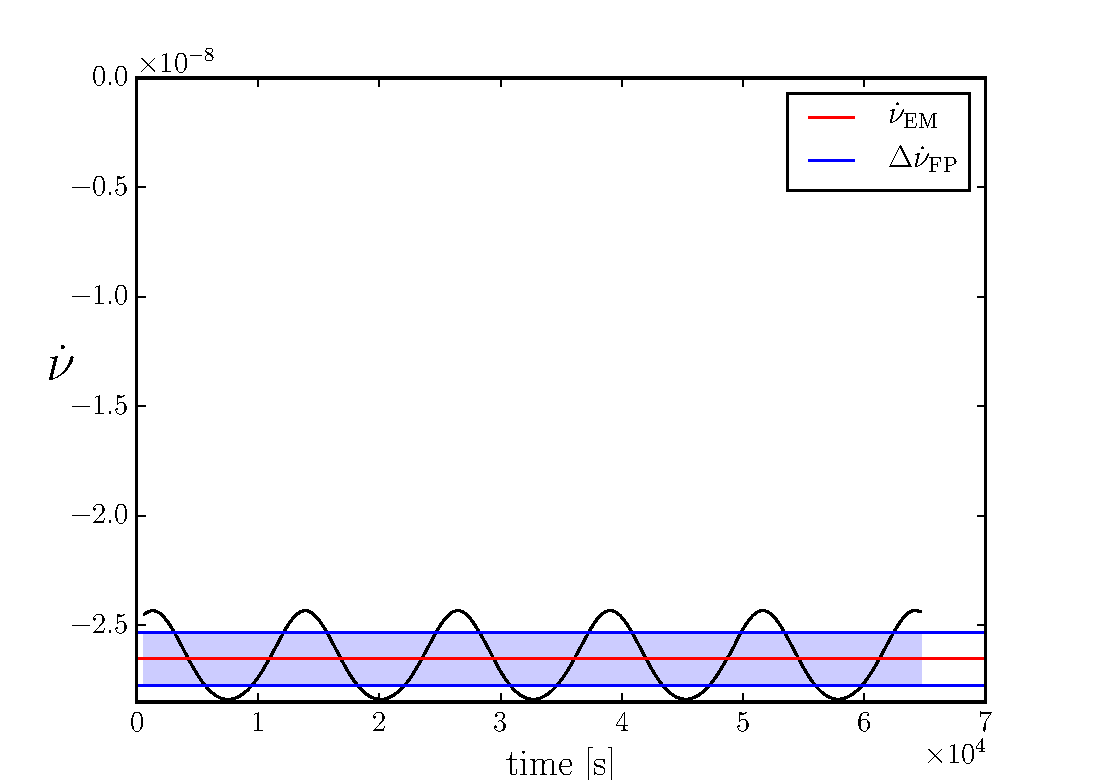
\includegraphics[width=0.5\textwidth]{nu_dot_with_torque.pdf}
}{%
  \caption{Modulation in the spin-down rate due to precession. The solid black line
indicates the numerical solution including a torque; the solid red line indicates
the approximate average spin-down rate due to the EM toque as calculated
from equation \eqref{eqn: spin-down initial EM chi}; the blue lines indicate
the magnitude of modulation about the average spin-down due to precession; finally
the red-dashed line is the prediction of equation \eqref{eqn: 1238}}
\label{fig: nu_dot with torque}
}
\capbtabbox{%
   \begin{tabular}{ccl}
\multicolumn{3}{c}{Simulation parameters} \\
\hline
$\omega_0$  &=& 10.0 rad/s\\
$B_0$  &=& $ 1.897\times 10^{14} $ G \\
$\chi$  &=& 60.00$^{\circ}$ \\
$a_0$ &=& 3.00$^{\circ}$ \\
$\tilde{\theta}$ &= & 3.05$^{\circ}$ \\
$\mathcal{A}_{\mathrm{EM}}$ &= & $0.42$
\end{tabular}
    
}{%
  \caption{}%
  \label{tab:}
}
\end{floatrow}
\end{figure}

\FloatBarrier

\subsubsection{EM torque amplification of the spin-down modulation}
When $\Aem$ is greater than unity the spin-down modulations are amplified by 
the torque. We can generate an analytic prediction for this by by inserting
eqn.~\eqref{eqn: Phi_dot} and \eqref{eqn: Theta} into the vacuum point-dipole spin-down
torque:
\begin{align}
    \ddot{\Phi} & = k \dot{\Phi}\sin^{2}\Theta \\
                &=-\frac{2R}{3c} \epsA 
    \left(\dot{\phi} +  \frac{\dot{\psi} \sin(\chi)(\cos\theta\sin\chi - \sin \psi \sin \theta \cos\chi)
    }{(\sin\theta \cos \chi - \cos \theta \sin \psi \sin \chi)^{2} + \cos^{2}\psi \sin^{2} \chi}\right)^{3}
    \sin^{2}\left(\cos^{-1}\left(\sin\theta\sin\psi\sin\chi + \cos\theta\cos\chi\right)\right)\\
    &=-\frac{2R}{3c} \epsA 
    \left(\dot{\phi} +  \frac{\dot{\psi} \sin(\chi)(\cos\theta\sin\chi - \sin \psi \sin \theta \cos\chi)
    }{(\sin\theta \cos \chi - \cos \theta \sin \psi \sin \chi)^{2} + \cos^{2}\psi \sin^{2} \chi}\right)^{3}
    \left(\sin\theta\sin\psi\sin\chi + \cos\theta\cos\chi\right)
\end{align}
where we are implicitly assuming $\theta=\mathrm{const.}$ which is still 
approximately true in the biaxial case \textcolor{red}{check this}.
Finally we assume that the Euler angles are approximately the same as in 
the torque free case, that is:
\begin{align}
    \phi(t) = \omega_{0}t + \phi_{0} &&& \psi(t) = -\epsI \omega_{0} t + \pi/2
\end{align}

 \begin{align}
     \ddot{\Phi} &=-\frac{2R}{3c} \omega_{0}^{3}\epsA
     \left(1 -  \epsI\frac{ \sin(\chi)(\cos\theta\sin\chi - \sin \psi \sin \theta \cos\chi)
     }{(\sin\theta \cos \chi - \cos \theta \sin \psi \sin \chi)^{2} + \cos^{2}\psi \sin^{2} \chi}\right)^{3}
     \left(\sin\theta\sin\psi\sin\chi + \cos\theta\cos\chi\right)
 \end{align}     
In figure \ref{fig: nu_dot with torque EM} we plot the results of a simulation
for which this amplifcation factor is greater than unity. This shows that the
spindown variations are given by \ref{eqn: spin-down variations FP EM} rather
than \eqref{eqn: spin-down variations FP}.

%\begin{figure}[ht]
%\centering
%	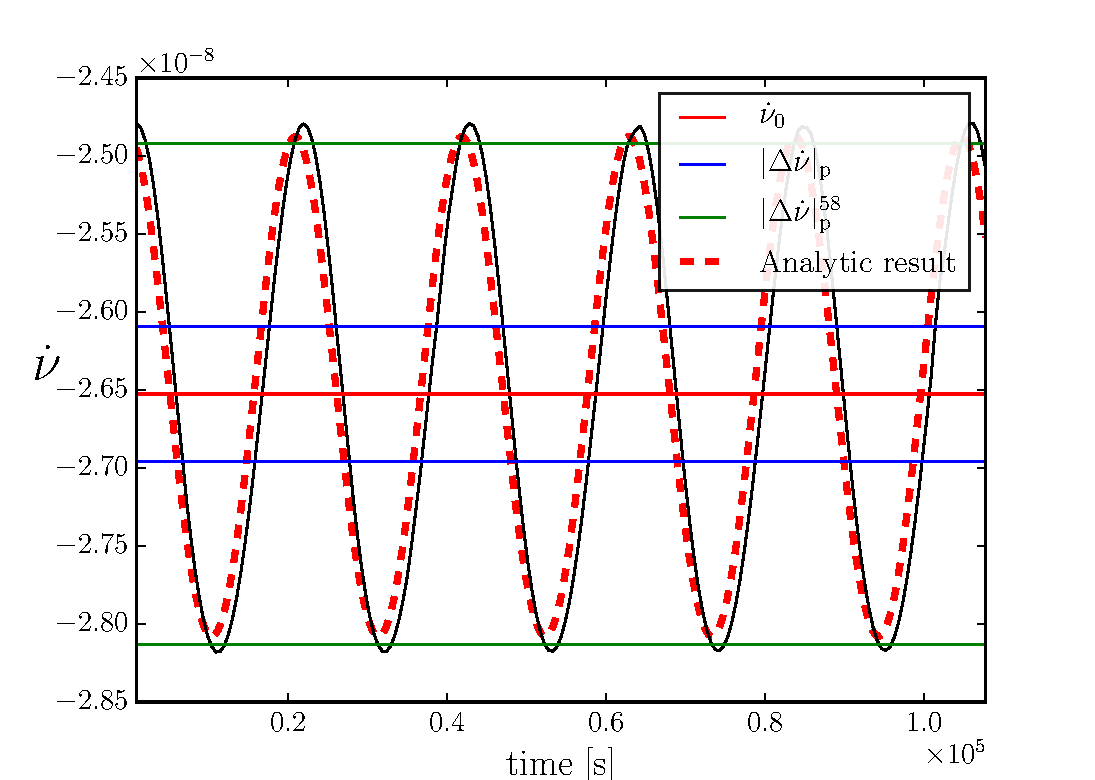
\includegraphics[width=0.5\textwidth]{nu_dot_with_torque_EM_amplification.pdf}
%\caption{EM amplification of the modulation in the spin-down rate due to precession. 
%    The solid black line
%indicates the numerical solution including a torque; the solid red line indicates
%the approximate average spin-down rate due to the EM toque as calculated
%from equation \eqref{eqn: spin-down initial EM chi}; the blue region indicates
%the modulation about the average spin-down due to precession from equation 
%\eqref{eqn: spin-down variations FP} while the green region indicates the modulation 
%about as calculated from equation \eqref{eqn: spin-down variations FP EM}.}
%\label{fig: nu_dot with torque EM}
%\end{figure}

\begin{figure}[htb]
\begin{floatrow}
\ffigbox{%
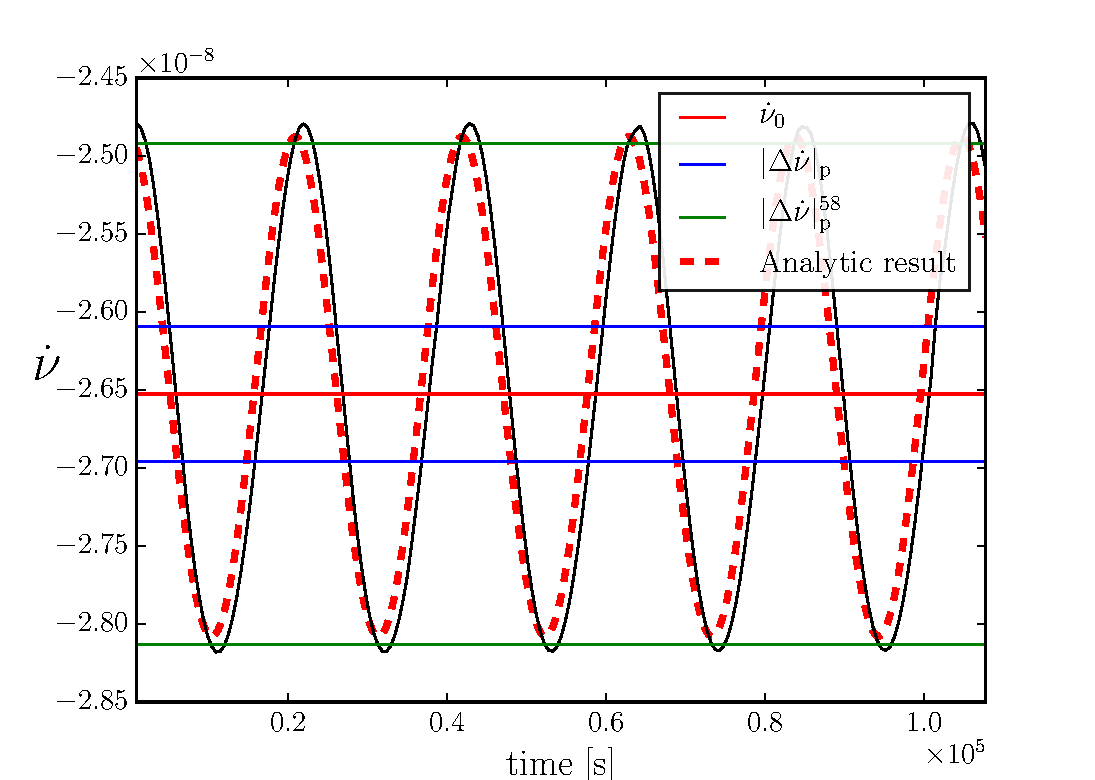
\includegraphics[width=0.5\textwidth]{nu_dot_with_torque_EM_amplification.pdf}
}{%
  \caption{EM amplification of the modulation in the spin-down rate due to precession. 
    The solid black line
indicates the numerical solution including a torque; the solid red line indicates
the approximate average spin-down rate due to the EM toque as calculated
from equation \eqref{eqn: spin-down initial EM chi}; the blue region indicates
the modulation about the average spin-down due to precession from equation 
\eqref{eqn: spin-down variations FP} while the green region indicates the modulation 
about as calculated from equation \eqref{eqn: spin-down variations FP EM}.}
\label{fig: nu_dot with torque EM}%
  \label{fig: nu_dot with torque EM}
}
\capbtabbox{%
   \begin{tabular}{ccl}
\multicolumn{3}{c}{Simulation parameters} \\
\hline
$\omega_0$  &=& 100.0 rad/s\\
$B_0$  &=& $ 1.897\times 10^{14} $ G \\
$\chi$  &=& 60.00$^{\circ}$ \\
$a_0$ &=& 3.00$^{\circ}$ \\
$\tilde{\theta}$ &= & 3.09$^{\circ}$ \\
$\mathcal{A}_{\mathrm{EM}}$ &= & $12.0$
\end{tabular}
    
}{%
  \caption{}%
  \label{tab:}
}
\end{floatrow}
\end{figure}

\FloatBarrier
\subsection{Double peaked spin-down values}


\biblio
\end{document}

